\section{Numerical Results}
\label{sec:experiments}

\subsection{Examples of running Simulated Annealing}

\begin{table}[h]
    \center
    \caption{Simulated Annealing with BR test to $\tau=10^{-7}$}
    \label{table:run_example}
    \footnotesize
    \setstretch{1.5}
    \begin{tabular}{c|cc|cc}
& $\vect{x}^\star$ & $f(\vect{x}^\star)$ & $\# f$ evals & $\# \nabla f$ evals \\
\hline
1 & ( 9.42478, 2.47500 ) & 0.39789 & 448 & 166 \\
2 & ( 9.42478, 2.47500 ) & 0.39789 & 607 & 224 \\
3 & ( 9.42478, 2.47500 ) & 0.39789 & 688 & 232 \\
4 & ( -3.14159, 12.27500 ) & 0.39789 & 567 & 167 \\
5 & ( -3.14159, 12.27500 ) & 0.39789 & 648 & 195 \\
6 & ( -3.14159, 12.27500 ) & 0.39789 & 568 & 199 \\
7 & ( 3.14159, 2.27500 ) & 0.39789 & 529 & 183 \\
8 & ( 3.14159, 2.27500 ) & 0.39789 & 486 & 172 \\
9 & ( 3.14159, 2.27500 ) & 0.39789 & 528 & 204 \\
10 & ( -3.14159, 12.27500 ) & 0.39789 & 527 & 190 \\
11 & ( 3.14159, 2.27500 ) & 0.39789 & 607 & 195 \\
12 & ( -3.14159, 12.27500 ) & 0.39789 & 568 & 201 \\
13 & ( -3.14159, 12.27500 ) & 0.39789 & 489 & 179 \\
14 & ( -3.14159, 12.27500 ) & 0.39789 & 608 & 203 \\
15 & ( 9.42478, 2.47500 ) & 0.39789 & 728 & 228 \\
16 & ( 3.14159, 2.27500 ) & 0.39789 & 528 & 179 \\
17 & ( 9.42478, 2.47500 ) & 0.39789 & 728 & 235 \\
18 & ( 3.14159, 2.27500 ) & 0.39789 & 567 & 201 \\
19 & ( 3.14159, 2.27500 ) & 0.39789 & 649 & 225 \\
20 & ( 3.14159, 2.27500 ) & 0.39789 & 767 & 244 \\
    \end{tabular}
    
    \vspace{10pt}

    \Cref{table:run_example}: note that all 3 global minima are found. The following parameters were used and serve as good
    default parameters: $L_0 = 20, \delta=1.1, \epsilon_s = 10^{-6}, \chi=0.9, \gamma=10^{-2}$ and
    $T=0.5$.
\end{table}

\begin{figure}
    \centering
    \caption{Average SA trajectories for BR}
    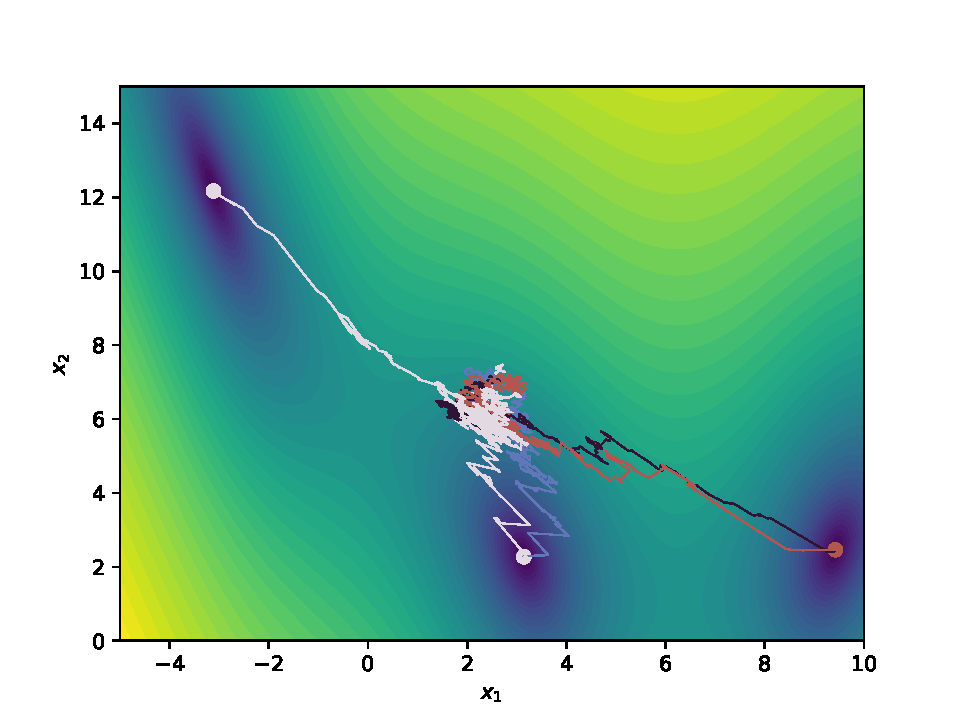
\includegraphics[scale=0.42]{figures/fig51-branin.pdf}
    \label{fig:5.1.1}
\end{figure}

\begin{figure}
    \centering
    \caption{Average SA trajectories for GP}
    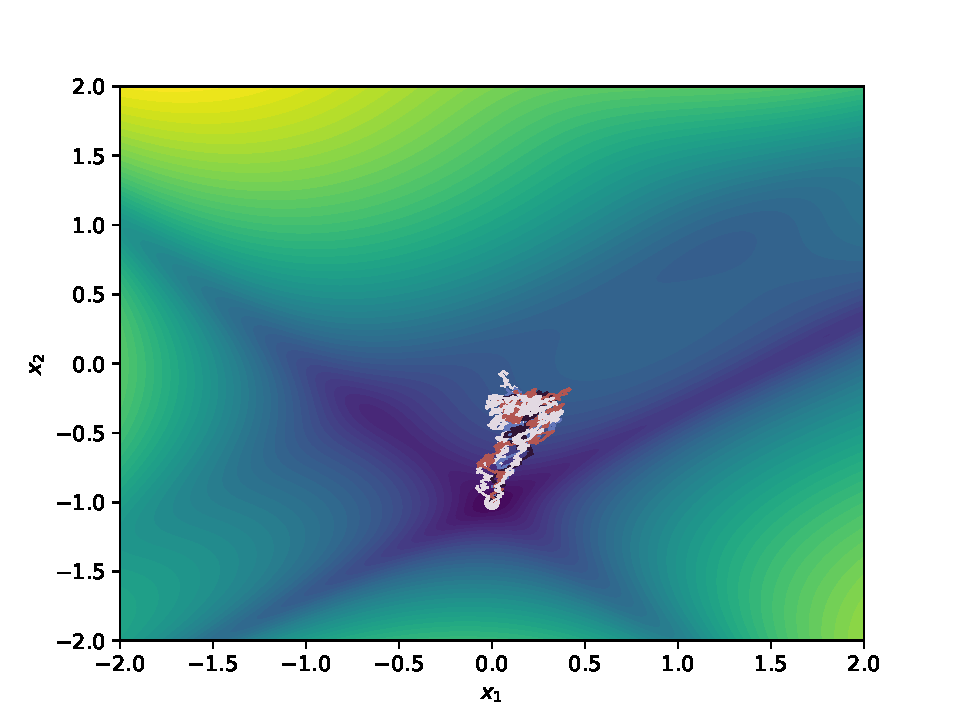
\includegraphics[scale=0.42]{figures/fig51-goldstein_price.pdf}
    \label{fig:5.1.2}
\end{figure}

\begin{table}
    \center
    \caption{Average number of runs required to solve problems}
    \label{table:run_numbers}
    \footnotesize
    \setstretch{1.5}
    \begin{tabular}{cc|cccc}
        & Problem & Avg. num runs & Solutions found & $\# f$ evals & $\# \nabla f$ evals \\
        \hline
1 & RB & 1.0 & 1 & 614.58 & 210.68 \\
1 & GP & 1.6 & 1 & 1072.38 & 385.96 \\
3 & BR & 5.18 & 3 & 3012.68 & 1041.06 \\
1 & H3 & 1.12 & 1 & 575.08 & 211.06 \\
1 & H6 & 1.58 & 1 & 737.7 & 284.1 \\
    \end{tabular}

\end{table}
    
\Cref{table:run_numbers} shows the average required number of runs for the benchmark problems RB, GP, BR, H3, and H6. Simulated Annealing is run
repeatedly until all known global minima are found for the problem. A solution $\hat{\vect{x}}_i$ is considered the same
if $|\hat{\vect{x}}_i - \vect{x}^\star_j|_2 \leq \tau = 10^{-4}$.
This process is repeated $M=50$ times
and the average number of runs, average function and Jacobian values are reported. In all cases, every global minimum
was found. The results show that test problems BR and H6 require a greater average number of required runs per global minima. 

The following
Simulated Annealing parameters were used: $l_0=20, \delta=1.1, \epsilon_s=1e-4, \chi=0.9,
\gamma=10^{-2}$, and $t=0.5$.


\begin{table}
    \center
    \caption{Global and local minima found by Simulated Annealing}
    \label{table:minima}
    \footnotesize
    \setstretch{1.5}
    \begin{tabular}{rc|lr}
        Prob & Type & $\vect{x}^\star_i$ & $f(\vect{x}^\star_i)$ \\
        \hline
RB & g & ( 1.0, 1.0 ) & 0.0 \\
\hline
GP & g & ( -0.0, -1.0 ) & 3.0 \\
& l &( -0.6, -0.4 ) & 30.0 \\
& & ( 1.8, 0.2 ) & 84.0 \\
\hline
BR & g & ( -3.14159, 12.275 ) & 0.39789 \\
& & ( 3.14159, 2.275 ) & 0.39789 \\
& & ( 9.42478, 2.475 ) & 0.39789 \\
\hline
H3 & g & ( 0.11461, 0.55565, 0.85255 ) & -3.86278 \\
& l &( 0.10934, 0.86052, 0.56412 ) & -3.08976 \\
\hline
H6 & g & ( 0.20169, 0.15001, 0.47687, 0.27533, 0.31165, 0.6573 ) & -3.32237 \\
& l &( 0.40465, 0.88244, 0.8461, 0.57399, 0.13893, 0.0385 ) & -3.20316 \\
\end{tabular}
\end{table}

\begin{figure}
    \center
    \caption{Markov chain trajectories for BR}
    \label{fig:markov-traj}
    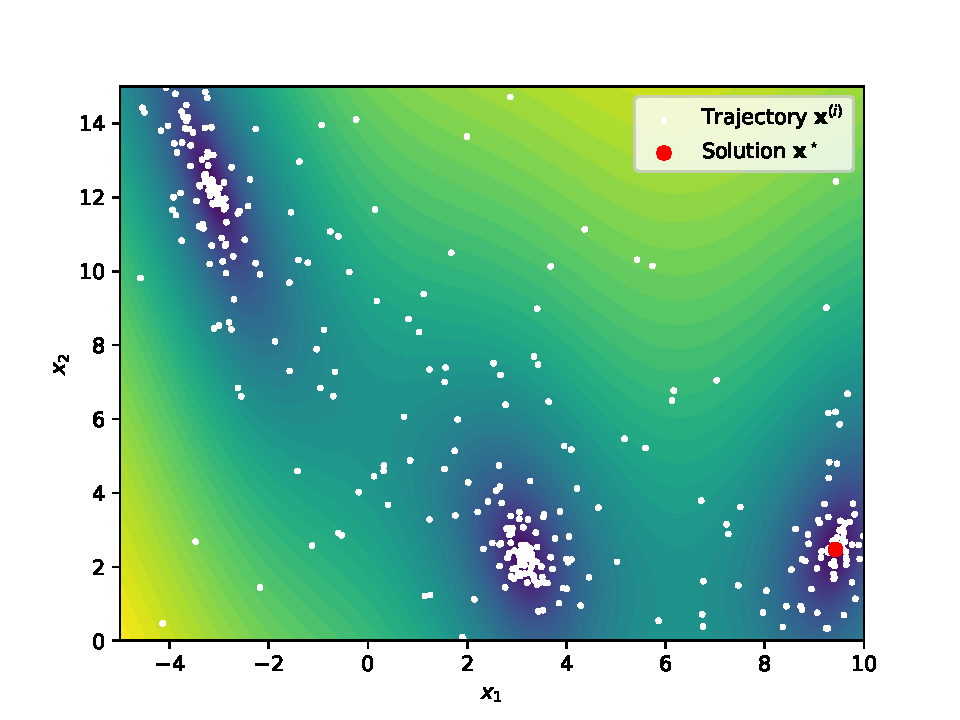
\includegraphics[scale=0.55]{figures/fig-traj.pdf}
    \vspace{10pt}
    \footnotesize
    \setstretch{1.2}
    \flushleft
    \textbf{\Cref{fig:markov-traj}} shows the effective sampling of the test function BR by the Simulated
    Annealing method. White points denote states visisted by the Markov chains. Red denotes the solution
    that this run converged to. Observe how SA oversamples points near the bottoms of the regions of attraction
    of each global minimum.
\end{figure}
